Para avaliar a eficácia do modelo de IA desenvolvido para o sistema, foram realizadas análises comparativas entre as predições geradas e os valores reais de produção de leite. Com o desenvolvimento da IA baseada no modelo Random Forest Regressor, o desempenho do sistema foi avaliado por meio do coeficiente de determinação (\(R^2\)), obtendo-se o valor de 0,73. Como mostrado no Gráfico \Cref{grph:example}, a dispersão das predições em relação aos valores reais indica que a maior parte das estimativas se aproxima da diagonal \(y = x\), evidenciando que o modelo consegue explicar 73\% da variabilidade observada na produção de leite. Apesar de alguns desvios individuais, os resultados demonstram que o sistema fornece previsões consistentes e confiáveis para o manejo do rebanho.  O modelo considera informações como dias em lactação, produção média de lactação, histórico da produção média, idade da búfala, idade no primeiro parto e intervalo entre partos, permitindo análises detalhadas e suporte à tomada de decisão baseada em dados.

\begin{graph}[!h]
\centering
\SetCaptionWidth{\ifbool{@LayoutA}{0.47}{0.49}\linewidth}
\caption{Dispersão das predições do modelo}%
\label{grph:example}
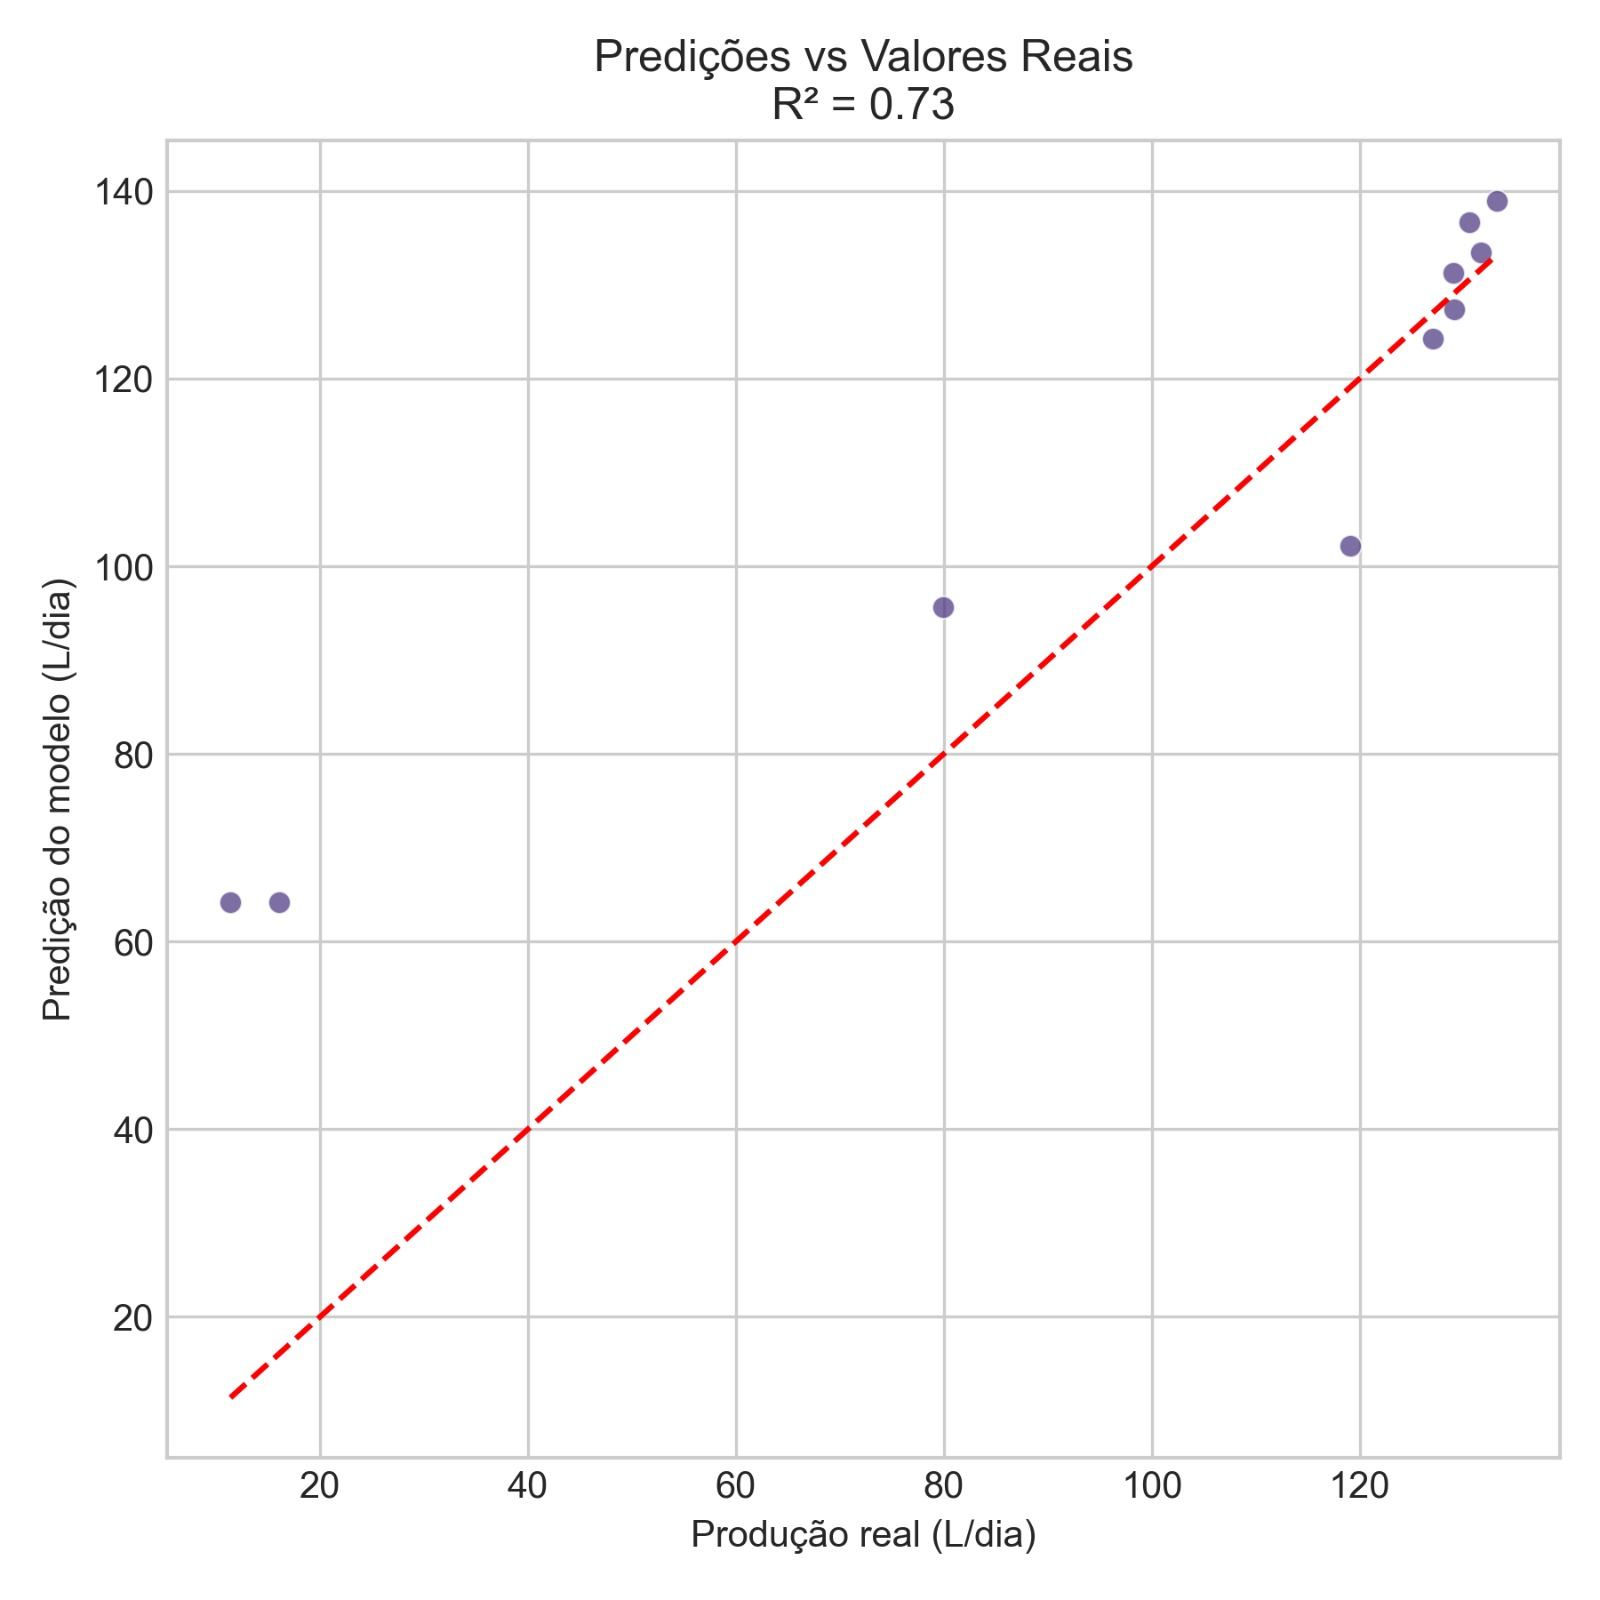
\includegraphics[width = \CaptionWidth]{R}
\SourceOrNote{Autoria Própria (2025)}
\end{graph}
